\title{CS313 : DataBases and Information Systems Lab \\
    \vspace{0.6cm}
    Lab Assignment 2
} % You may change the title if you want.
% \subtitle{Hello}
\author{Sourabh Bhosale \\ 200010004}

\date{\today}

\documentclass[12pt]{article}
\usepackage{fullpage}
\usepackage{enumitem}
\usepackage{amsmath,mathtools}
\usepackage{amssymb}
\usepackage[super]{nth}
\usepackage{textcomp}
\usepackage{hyperref}
\usepackage{multicol}
\usepackage{multirow}
\usepackage{minted}
% \usepackage{fontspec}
% \usepackage[showframe]{geometry}

% \usepackage[default]{sourcesanspro}
% \usepackage[T1]{fontenc}

% \usepackage[sfdefault]{noto}
% \usepackage[T1]{fontenc}

\usepackage[default,oldstyle,scale=0.95]{opensans} %% Alternatively
%% use the option 'defaultsans' instead of 'default' to replace the
%% sans serif font only.
\usepackage[T1]{fontenc}

% \setmainfont{Roboto}
\usepackage{titling}
\hypersetup{
    colorlinks=true,
    linkcolor=blue,
    filecolor=magenta,      
    urlcolor=cyan,
}

\renewcommand\maketitlehooka{\null\mbox{}\vfill}
\renewcommand\maketitlehookd{\vfill\null}

\begin{document}


\begin{titlingpage}
\maketitle
\end{titlingpage}

\newpage
%---------------------------------------------------------------------

% \begin{tiny}
\section{Table-wise all integrity constraints}
\begin{figure}[!hbt]
    \centering
    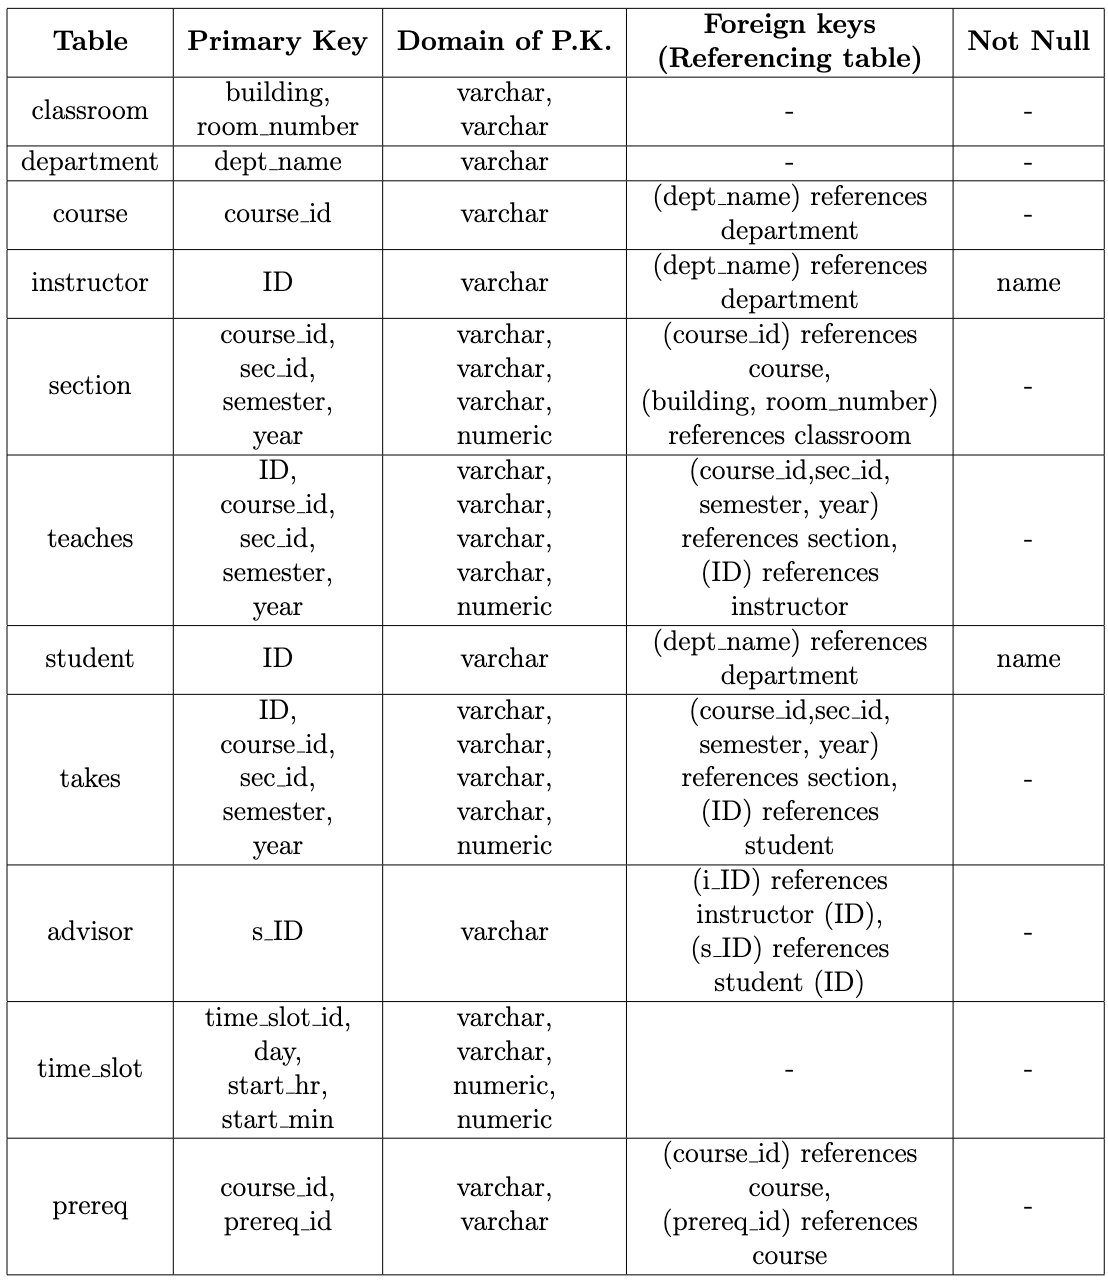
\includegraphics[scale=0.68]{screenshots/table_1.png}
    \label{fig:my_label1}
    \caption{\centering{All integrity constraints for different tables \\ (Primary key, Domain of Primary key, Foreign key and Not Null)}}
\end{figure}


%  \begin{table}[hbt]
%     \centering
%     \begin{tabular}{|c|c|c|c|c|}
 
%         \hline
%         \textbf{Table} & \textbf{Primary Key} & \textbf{Domain of P.K.} & \textbf{\begin{tabular}[c]{@{}c@{}}Foreign keys\\(Referencing table) \end{tabular}} & \textbf{Not Null}  \\  
        
%         %%%%%%%%%%%%%%%%%
%         \hline
%         %  \multirow{2}{*}{classroom} & building & VARCHAR(15) & \multirow{2}{*}{-}& \multirow{2}{*}{-}\\ \cline{2-3}
%         %  & room\_number & VARCHAR(7) & & \\ \hline
%         %  department & dept\_name & VARCHAR(20) & - & - \\ 
%         % \hline
        
%         %%%%%%%%%%%%%%%%%
%         classroom & 
%         \begin{tabular}[c]{@{}c@{}}building,\\room\_number \end{tabular} & 
%         \begin{tabular}[c]{@{}c@{}}varchar,\\varchar \end{tabular} &
%         - & 
%         - \\  
%         \hline
        
%         department & 
%         dept\_name & 
%         varchar & 
%         - & 
%         - \\  
%         \hline
        
%         course & 
%         course\_id & 
%         varchar & 
%         \begin{tabular}[c]{@{}c@{}}(dept\_name) references\\ department \end{tabular} & - \\ 
%         \hline
        
%         instructor & 
%         ID & 
%         varchar & 
%         \begin{tabular}[c]{@{}c@{}}(dept\_name) references\\ department \end{tabular} & name \\  
%         \hline
        
%         section & 
%         \begin{tabular}[c]{@{}c@{}}course\_id,\\ sec\_id,\\ semester,\\year\end{tabular} &
%         \begin{tabular}[c]{@{}c@{}}varchar,\\varchar,\\varchar,\\numeric \end{tabular} &
%         \begin{tabular}[c]{@{}c@{}}(course\_id) references \\ course, \\ (building, room\_number) \\ references classroom\end{tabular}  &
%         - \\  
%         \hline
        
%         teaches & 
%         \begin{tabular}[c]{@{}c@{}}ID,\\course\_id,\\sec\_id,\\semester,\\year \end{tabular} &
%         \begin{tabular}[c]{@{}c@{}}varchar,\\varchar,\\varchar,\\varchar,\\numeric \end{tabular} &
%         \begin{tabular}[c]{@{}c@{}}(course\_id,sec\_id,\\semester, year)\\references section,\\(ID) references\\ instructor \end{tabular} & 
%         - \\  
%         \hline
        
%         student &
%         ID & 
%         varchar & 
%         \begin{tabular}[c]{@{}c@{}}(dept\_name) references\\ department \end{tabular} & 
%         name \\  
%         \hline
        
%         takes &
%         \begin{tabular}[c]{@{}c@{}}ID,\\course\_id,\\sec\_id,\\semester,\\year \end{tabular} &
%         \begin{tabular}[c]{@{}c@{}}varchar,\\varchar,\\varchar,\\varchar,\\numeric \end{tabular} & 
%         \begin{tabular}[c]{@{}c@{}}(course\_id,sec\_id,\\semester, year)\\references section,\\(ID) references\\student \end{tabular} & 
%         - \\  
%         \hline
        
%         advisor & 
%         s\_ID & 
%         varchar & 
%         \begin{tabular}[c]{@{}c@{}}(i\_ID) references\\instructor (ID),\\(s\_ID) references\\student (ID) \end{tabular} & 
%         -  \\  
%         \hline
        
%         time\_slot &
%         \begin{tabular}[c]{@{}c@{}}time\_slot\_id,\\day,\\start\_hr,\\start\_min\end{tabular} &
%         \begin{tabular}[c]{@{}c@{}}varchar,\\varchar,\\numeric,\\numeric \end{tabular} &
%         - & 
%         - \\
%         \hline
        
%         prereq & 
%         \begin{tabular}[c]{@{}c@{}}course\_id,\\prereq\_id \end{tabular} & 
%         \begin{tabular}[c]{@{}c@{}}varchar,\\varchar\end{tabular} & 
%         \begin{tabular}[c]{@{}c@{}}(course\_id) references\\course,\\(prereq\_id) references\\course \end{tabular} &
%         - \\  
%         \hline
%     \end{tabular}
%     \caption{All integrity constraints (Primary key, Domain of Primary key, Foreign key and Not Null)}
%     \label{table1}
% \end{table}

% \end{tiny}

%---------------------------------------------------------------------

\newpage

\section{Student profile}
Here, full profile of the student using the tables student, department, takes, advisor and instructor is made.

\subsection{First approach}
Sorting of all the columns is done here without any repetitions using the given tables.
\\ \\
\textbf{Query:} \\
\fbox{ \begin{minipage}{40em}
\inputminted{mysql}{problem2a.sql}
\end{minipage}
}
\\ \\
\textbf{Output:}
\begin{figure}[hbt]
    \centering
    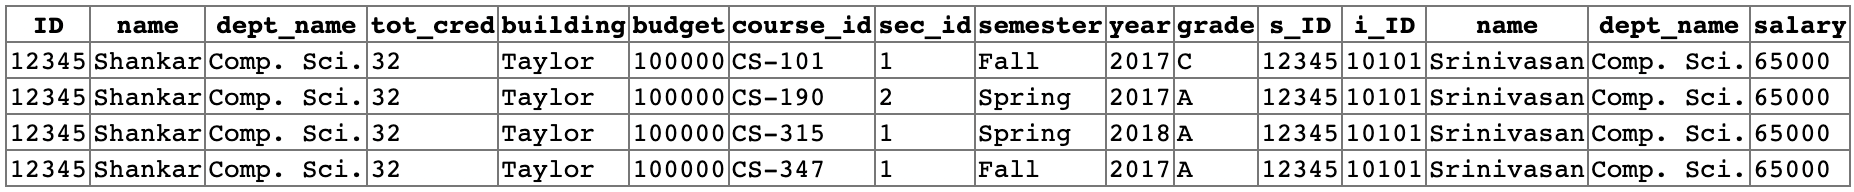
\includegraphics[scale=0.55]{screenshots/problem2a.png}
    \label{fig:my_label1}
\end{figure}

\subsection{Alternate approach}
Sorting of all the columns is done here according to the example output given in the assignment question.
\\ \\
\textbf{Query:} \\
\fbox{ \begin{minipage}{40em}
\inputminted{mysql}{problem2b.sql}
\end{minipage}
}
\\ \\
\textbf{Output:}
\begin{figure}[hbt]
    \centering
    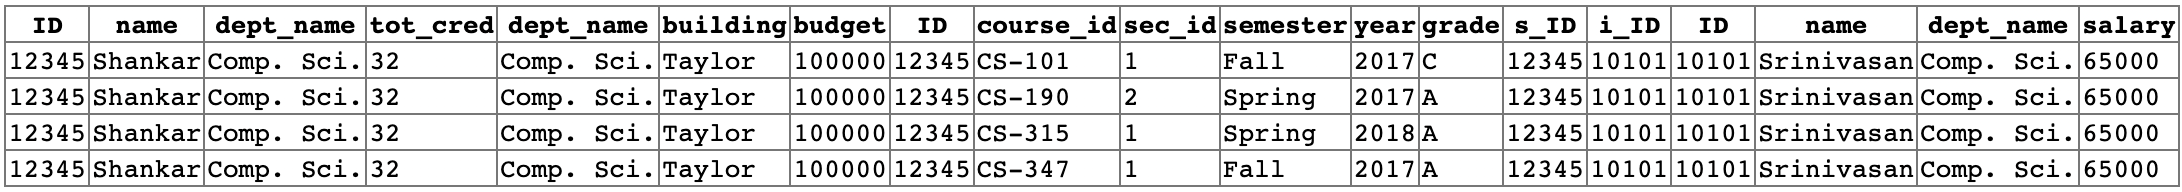
\includegraphics[scale=0.47]{screenshots/problem2b.png}
    \label{fig:my_label1}
\end{figure}

{\noindent In both places, you can change the \textit{student.ID} value accordingly.}

%---------------------------------------------------------------------

\section{Trying out \textit{select} and \textit{insert} on all the tables}
\subsection{Query}
% \textbf{Query:} \\ \\
\fbox{ \begin{minipage}{40em}
\inputminted{mysql}{problem3.sql}
\end{minipage}
}

\newpage

\subsection{Results}
You can see the new inputs in the last row of each table.
% \begin{figure}[hbt]
%  \subfigure[first image]{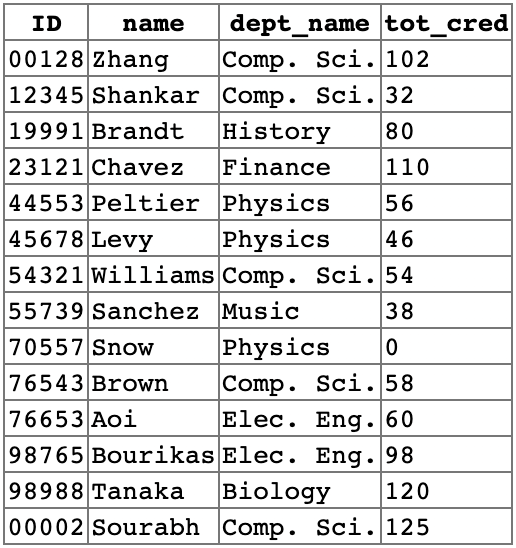
\includegraphics[scale=0.8]{screenshots/student.png}\label{first}}
%  \subfigure[second image]{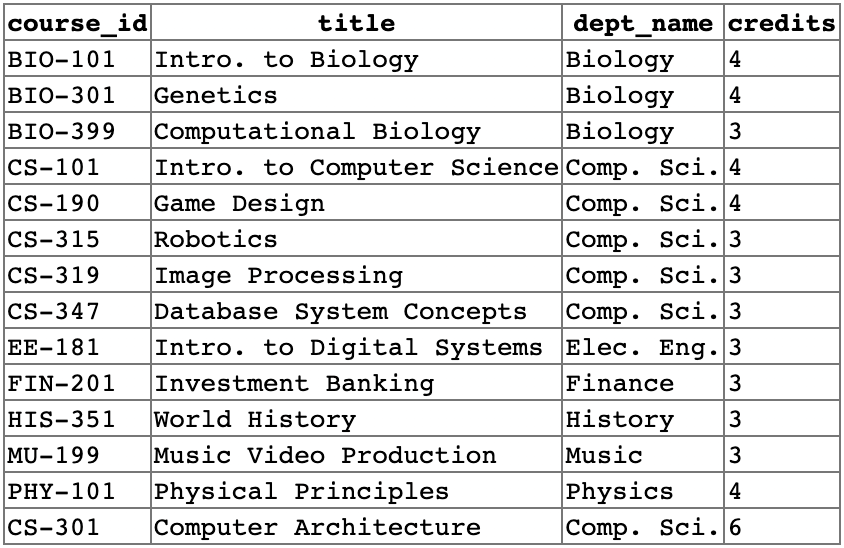
\includegraphics[scale=0.8]{screenshots/course.png}\label{second}}
%  \subfigure[second image]{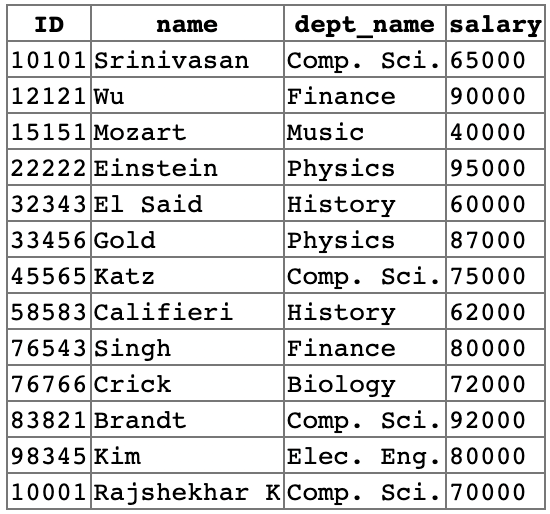
\includegraphics[scale=0.8]{screenshots/instructor.png}\label{second}}
%  \subfigure[second image]{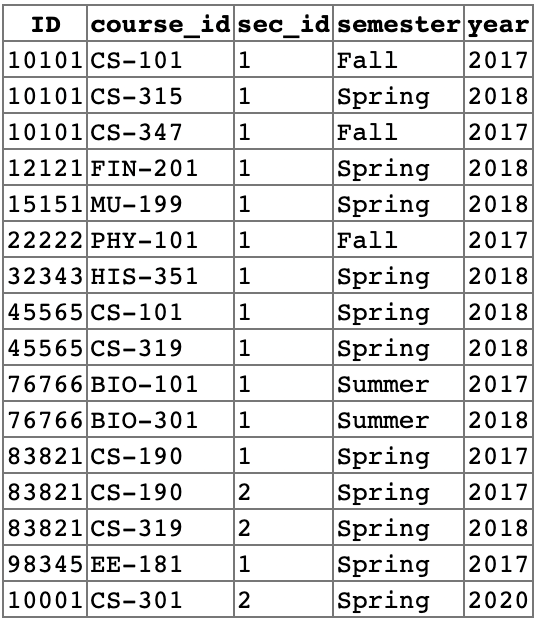
\includegraphics[scale=0.8]{screenshots/teaches.png}\label{second}}
%  \subfigure[second image]{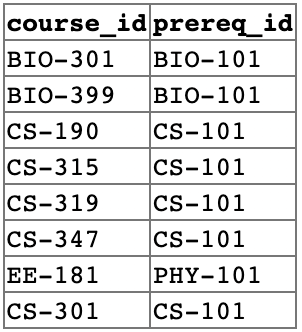
\includegraphics[scale=0.8]{screenshots/prereq.png}\label{second}}
%  \subfigure[second image]{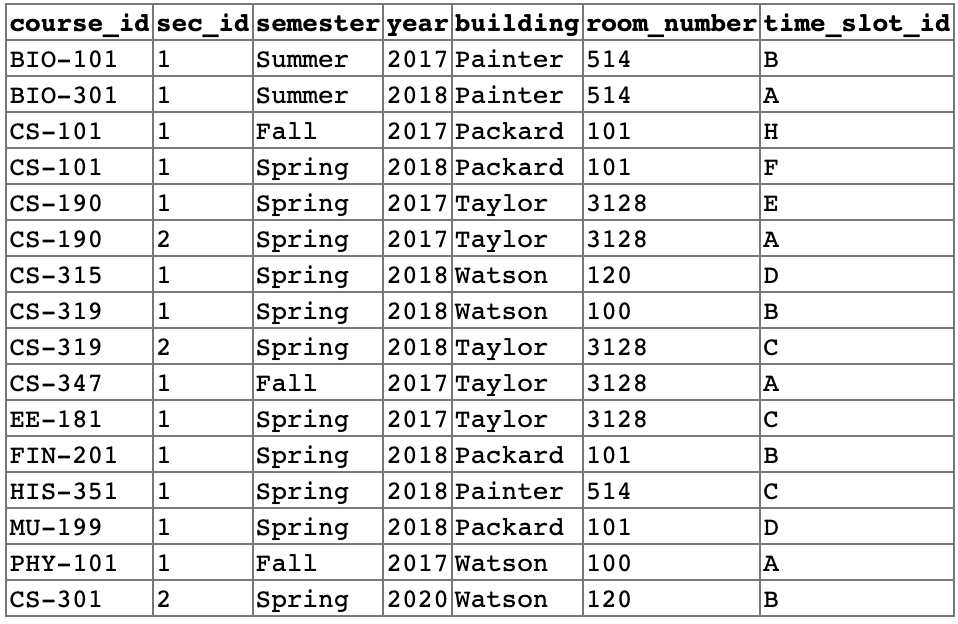
\includegraphics[scale=0.8]{screenshots/section.png}\label{second}}
%  \subfigure[second image]{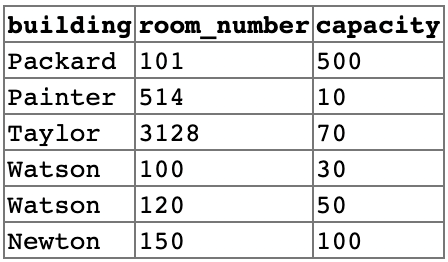
\includegraphics[scale=0.8]{screenshots/classroom.png}\label{second}}
%  \subfigure[second image]{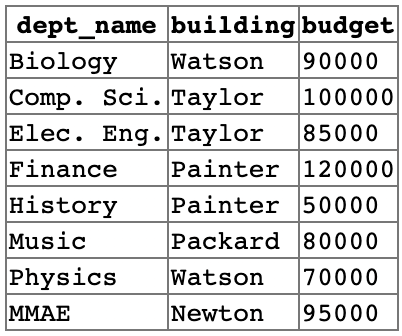
\includegraphics[scale=0.8]{screenshots/department.png}\label{second}}
%  \subfigure[second image]{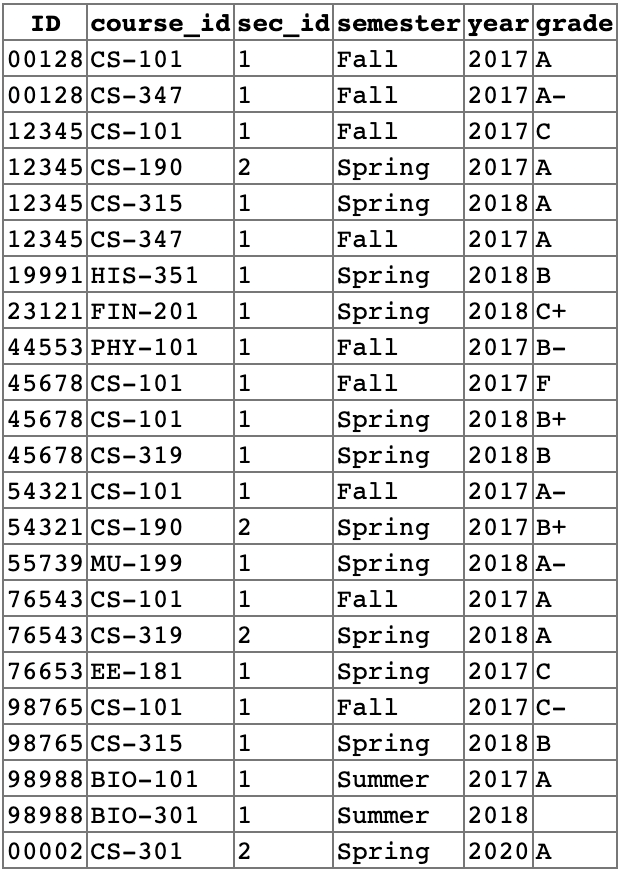
\includegraphics[scale=0.8]{screenshots/takes.png}\label{second}}
%  \subfigure[second image]{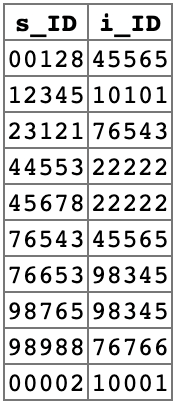
\includegraphics[scale=0.8]{screenshots/advisor.png}\label{second}}
%  \subfigure[second image]{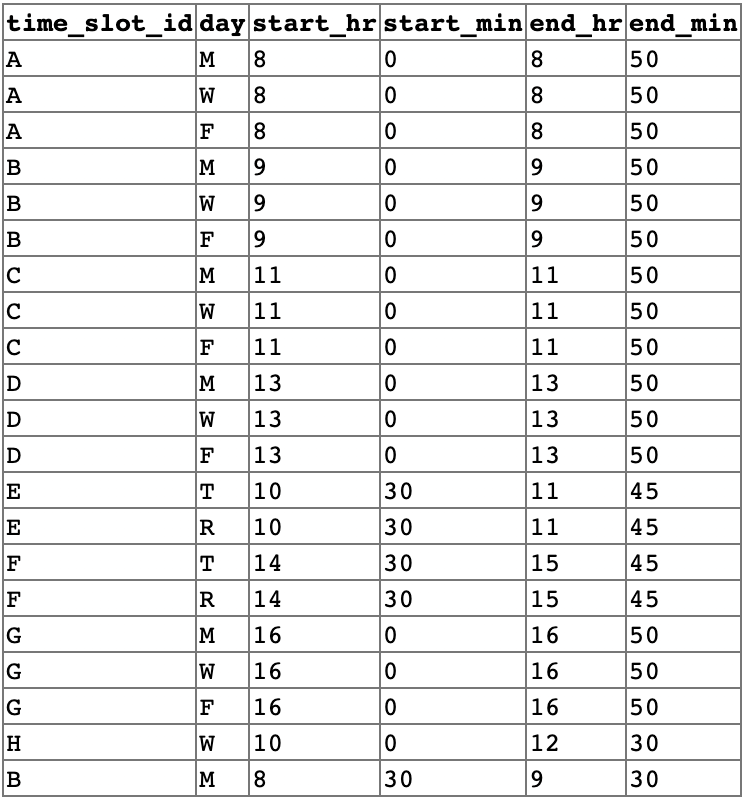
\includegraphics[scale=0.8]{screenshots/time_slot.png}\label{second}}
%  \caption{main caption}\label{main_label}
% \end{figure}

\begin{figure}[!hbt]
    \centering
    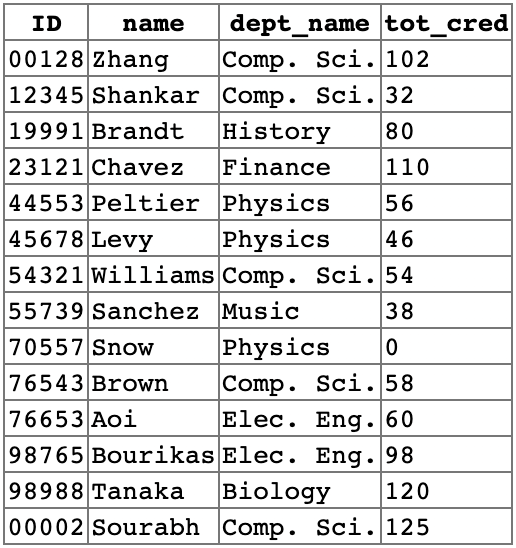
\includegraphics[scale=0.9]{screenshots/student.png}
    \label{fig:my_label1}
    \caption{Student table after insertion}
\end{figure}

\begin{figure}[!hbt]
    \centering
    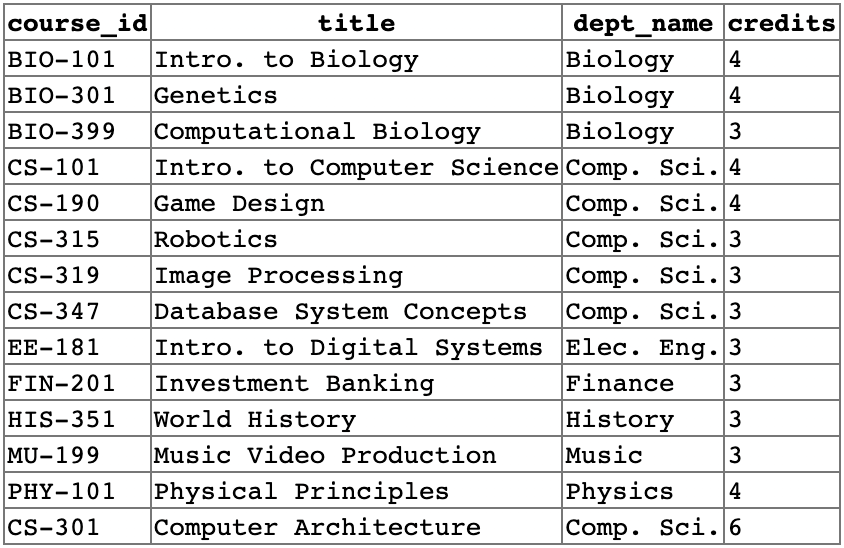
\includegraphics[scale=0.8]{screenshots/course.png}
    \label{fig:my_label1}
    \caption{Course table after insertion}
\end{figure}
\newpage

\begin{figure}[!hbt]
    \centering
    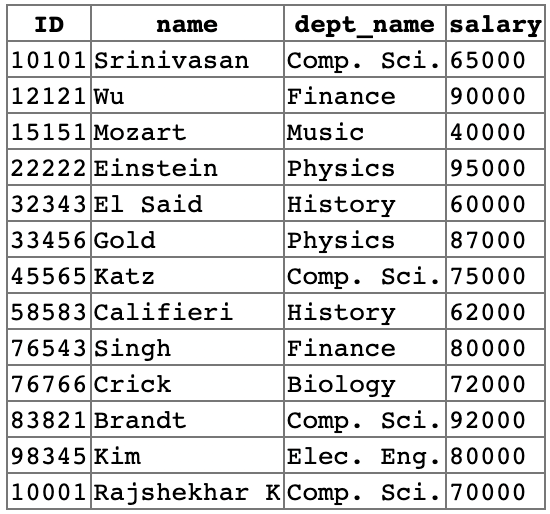
\includegraphics[scale=0.9]{screenshots/instructor.png}
    \label{fig:my_label1}
    \caption{Instructor table after insertion}
\end{figure}

\begin{figure}[!hbt]
    \centering
    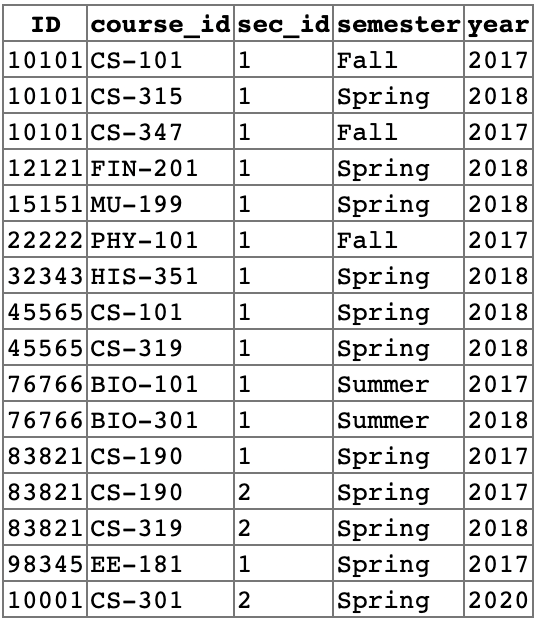
\includegraphics[scale=0.9]{screenshots/teaches.png}
    \label{fig:my_label1}
    \caption{Teaches table after insertion}
\end{figure}
\newpage

\begin{figure}[!hbt]
    \centering
    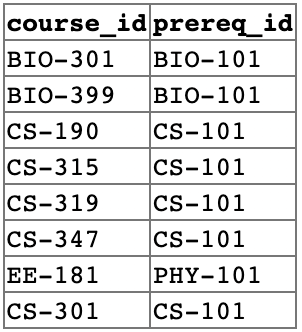
\includegraphics[scale=1.3]{screenshots/prereq.png}
    \label{fig:my_label1}
    \caption{Prereq table after insertion}
\end{figure}

\begin{figure}[!hbt]
    \centering
    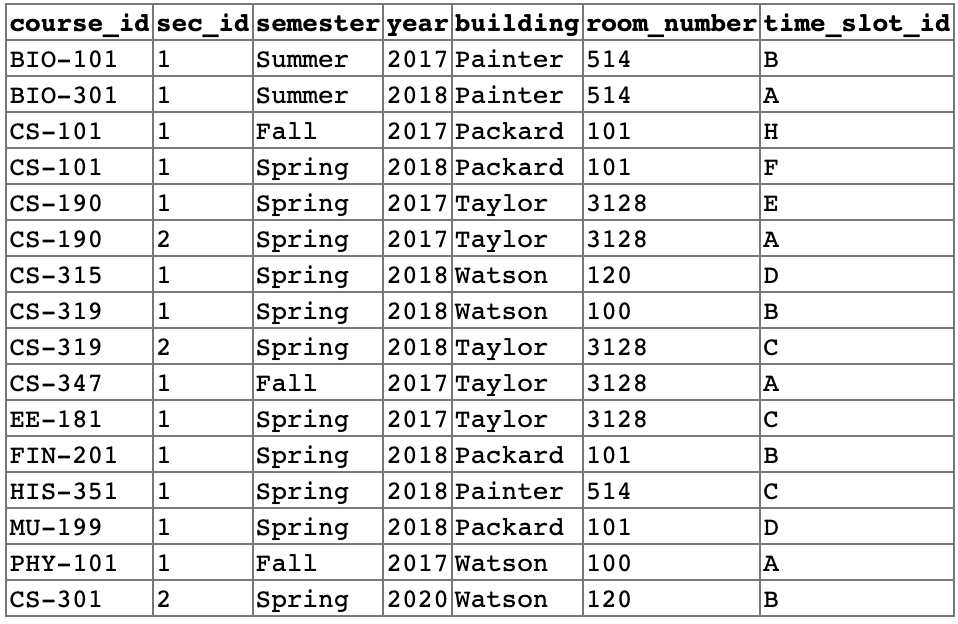
\includegraphics[scale=0.95]{screenshots/section.png}
    \label{fig:my_label1}
    \caption{Section table after insertion}
\end{figure}
\newpage

\begin{figure}[!hbt]
    \centering
    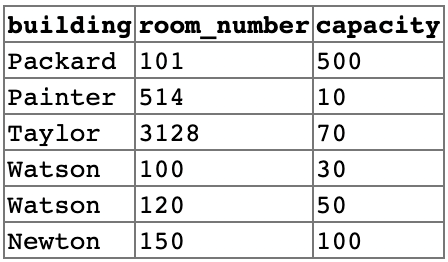
\includegraphics[scale=1.7]{screenshots/classroom.png}
    \label{fig:my_label1}
    \caption{Classroom table after insertion}
\end{figure}

\begin{figure}[!hbt]
    \centering
    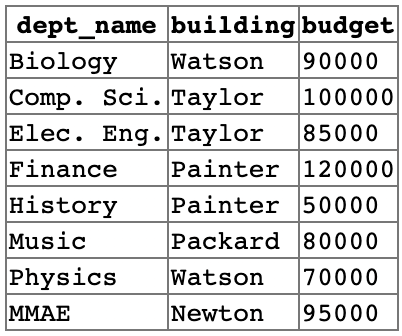
\includegraphics[scale=1.7]{screenshots/department.png}
    \label{fig:my_label1}
    \caption{Department table after insertion}
\end{figure}
\newpage

\begin{figure}[!hbt]
    \centering
    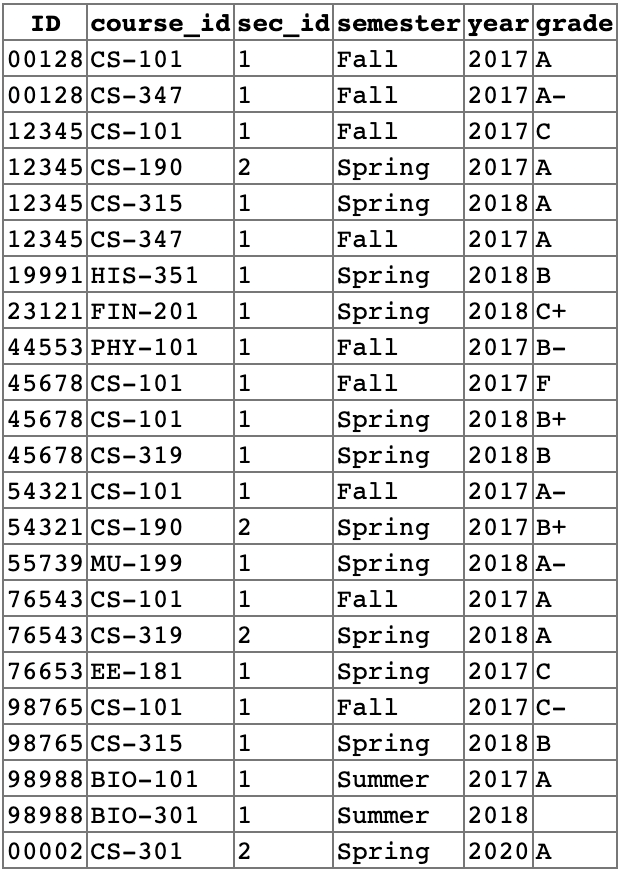
\includegraphics[scale=1.3]{screenshots/takes.png}
    \label{fig:my_label1}
    \caption{Takes table after insertion}
\end{figure}
\newpage

\begin{figure}[!hbt]
    \centering
    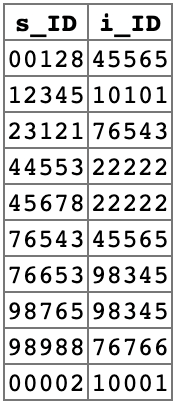
\includegraphics[scale=0.9]{screenshots/advisor.png}
    \label{fig:my_label1}
    \caption{Advisor table after insertion}
\end{figure}

\begin{figure}[!hbt]
    \centering
    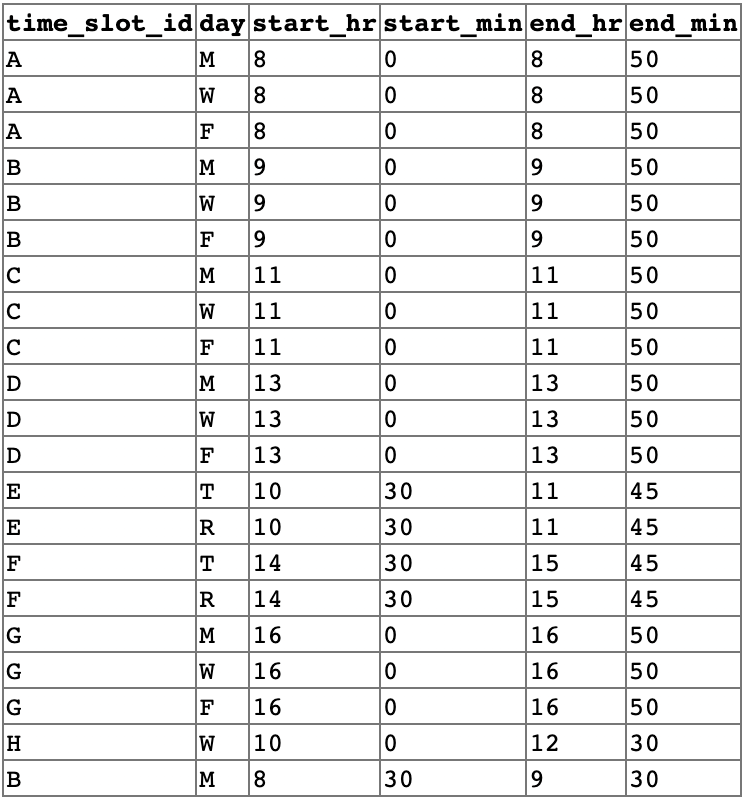
\includegraphics[scale=0.85]{screenshots/time_slot.png}
    \label{fig:my_label1}
    \caption{Time\_slot table after insertion}
\end{figure}
\newpage

%--------------------------------------------------------------

\section{Additional queries}

\subsection{Students (ID and names) from xxx department who have done courses from a room in building yyy}

\subsubsection{First Approach}
Here, we will refer \textit{section} and \textit{takes} table to see which courses a student takes then will filter out building-wise. \\
\textbf{Query:} \\ \\
\fbox{ \begin{minipage}{40em}
\inputminted{mysql}{problem4aa.sql}
\end{minipage}
}
\\ \\
\textbf{Output:}
\begin{figure}[!hbt]
    \centering
    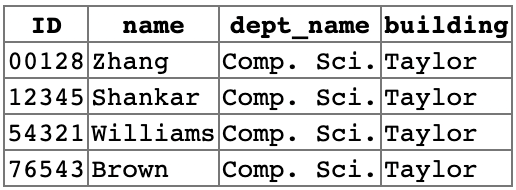
\includegraphics[scale=0.8]{screenshots/problem4aa.png}
    \label{fig:my_label1}
\end{figure}

\subsubsection{Another Approach}
Here, we will refer only \textit{student} and \textit{department} to collect data regarding buildings. \\
\textbf{Query:} \\ \\
\fbox{ \begin{minipage}{40em}
\inputminted{mysql}{problem4ab.sql}
\end{minipage}
}
\\ \\
\textbf{Output:}
\begin{figure}[!hbt]
    \centering
    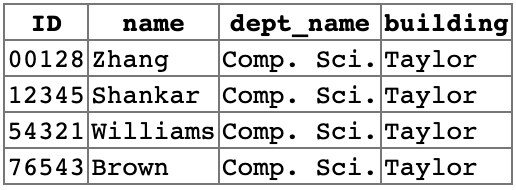
\includegraphics[scale=0.8]{screenshots/problem4ab.png}
    \label{fig:my_label1}
\end{figure}
\newpage

\subsection{Students who have A grade as well as a C grade}
\textbf{Query:} \\ \\
\fbox{ \begin{minipage}{40em}
\inputminted[obeytabs=true]{mysql}{problem4b.sql}
\end{minipage}
}
\\ \\
\textbf{Output:}
\begin{figure}[hbt]
    \centering
    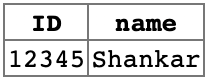
\includegraphics[scale=1.2]{screenshots/problem4b.png}
    \label{fig:my_label1}
\end{figure}

\subsection{All buildings and rooms which have classes on Wednesday}
 
\textbf{Query:} \\ \\
\fbox{ \begin{minipage}{40em}
\inputminted{mysql}{problem4c.sql}
\end{minipage}
}
\\ \\
\textbf{Output:}
\begin{figure}[hbt]
    \centering
    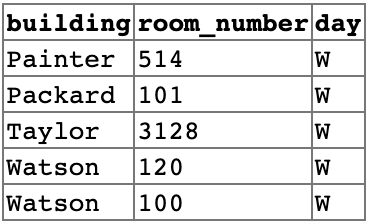
\includegraphics[scale=1.2]{screenshots/problem4c.png}
    \label{fig:my_label1}
\end{figure}

\end{document}